\chapter{先行研究}
\label{chap:search}

 睡眠の研究は近年注目を浴びている。睡眠に関連する研究の中の多くはbeddit、Bed Prssure Mat、やiSleepなどのように睡眠のモニタリングに関連したものである。一方本研究で開発をしたiOSアプリTokimekiDreamは、睡眠中に人が夢を見る習慣を利用して拡張現実の体験を促すために製作された。
 本章では睡眠のモニタリングを目的として製作された製品と、明晰夢を促進するデバイス両方においての先行事例・研究を紹介しのちに、複数の観点からTokimekiDreamとの比較を行い、新しい解決方法について提起する。

\section{モニタリング}
 本研究では睡眠を拡張現実を体験するための手段として注目した研究である。よって正確に睡眠をモニタリングする方法を探究するのは、この論文の課題ではない。しかし、明晰夢に影響を与えるのに夢をみる時間帯であるREM睡眠を感知することは重要な鍵となる。よって先行研究がどのように睡眠を感知しているのかについて次の章で述べる。そのあとに睡眠に影響を与えることで夢を操作することを目標としている製品について述べ、TokimekiDreamの参考にしたいと考えた。

\subsection{beddit}
\begin{itemize}
\item モニタリング手法:心拍数(鼓動によって起きる血流の変化を力センサーで完治)呼吸(呼吸に伴う肺の動きをセンサーで完治)\cite{beddit}
\item 正確性:46人を対象に実験し、心電計と比べた結果bedditの結果が99.94%の相関性があると証明されている
\item 目的:睡眠の質をビジュアライズ化させること
\item 優れた点:ウェラブルデバイズでないため、ユーザーが使用しやすい
\item 値段:18966円
\end{itemize}

\subsection{NEUROON TECHNOLOGY}
\begin{itemize}
\item モニタリング手法:脳波、眼球の動き、心拍数、血液中の酸素量、加速度、体動と体温 \cite{neuroon}
\item 正確性:商業目的の製品のため詳しいデーターは明かされていない
計と比べた結果bedditの結果が99.94%の相関性があると証明されている
\item 目的:不眠症などの睡眠に関する問題を解決するため
\item 優れた点:脳波を含んでいるということで、正確性が高いはず
\item 値段:36478円
\end{itemize}

\subsection{Zero}
\begin{itemize}
\item モニタリング方法:脳波 \cite{beWellApp}
\item 正確性:睡眠のモニタリング方法としてもっとも正確とされている
\item 目的:睡眠時無呼吸症候群の解決
\item 優れた点:睡眠の各ステージを正確に突き止めることができ、正確性は高いが、頭に装着しなければならないデバイスなのでユーザーの負担になる、寝るときにアプリに伝えないといけない、生活パターンを変えないといけない、汗をかきやすい、長期的な利用には向いていない
\item 値段:商業用目的ではないため不明
\end{itemize}

\subsection{Be Well App}
\begin{itemize}
\item モニタリング手法:ユーザーによるインプットは一切必要なく、ユーザーの充電、加速度からスマートフォン利用頻度・時間を測定、静けさ、部屋の明るさなどから、睡眠スタイルを検知する。 \cite{beWellApp}
\item 効果:8人の被験者に、Jawbone、Zeoと、BESモデルのアプリを試してもらい、全ての人がユーザー体験を過ごせたと結果がきた。
\item 正確性:睡眠時間+-42分
\item 目的:睡眠の長さを測ることで、うつ病、心配性、不眠症、高血圧になりにくい生活習慣へと導く
\item 優れた点:アプリという形で多くの人に実験をしてもらえる、ユーザーは普段の生活となんら変わりなく、過ごせるため、負担がかからない
\item 値段:商業用目的ではないため不明
\end{itemize}

\subsection{iSleep}
\begin{itemize}
\item モニタリング手法:スマートフォンに備わっている音声録音機能で体動、咳や、いびきなどを測定。 \cite{iSleep}
\item 正確性:被験者7人51日間の睡眠で90\%の正確性
\item 目的:健康向上のために睡眠時間とその質を正確に測定する
\item 優れた点:アプリをダウンロードするだけで簡単に使えるインターフェース。ローンチ10日間で100人のユーザーから睡眠に関する詳細なデータを集めることができた。
\item 値段:361円
\end{itemize}

\section{睡眠に対するインプット}

\subsection{sleepSheep}
\begin{itemize}
\item 目的:睡眠と光や音との関係性を活用し睡眠深度に即 した刺激を与える抱き枕型のインタフェースの提案 \cite{sleepSheep}
\item 正確性:モニタリングについてはアプリと照合されてある程度の正確性は証明されているが、光の部分については実験結果が明らかになっていない。
\item インプット:睡眠にゆかりのあるインターフェースである枕の改良を行うことで、新しいインタフェースの提案をしているが、その効果は実証されていない。
\item 値段:商業用目的ではないため不明
\end{itemize}


\subsection{takaratomi}
\begin{itemize}
\item 目的:みたい「夢」のイメージに近づけるように手助けをする。自分のための気分転換や、充実した楽しい時間を作り出す。 \cite{takaratomi}
\item 正確性:モニタリングについてはアプリと照合されてある程度の正確性は証明されているが、光の部分については実験結果が明らかになっていない。
\item インプット:視覚情報入力機能:みたい夢に関連した写真や画像を本体正面のパネル部分に貼り付けます。眠る前に視覚からのイメージを植え付けるもので、寝る直前にこの写真や画像を見つめ、頭のなかに十分イメージしたら就寝する。芳香剤発生機能:リラクセーション効果のある香りを発生させ、眠 りに適した状態に導く。BGM機能:眠りの導入時、予め選んで設定しておいた「恋愛」や「勇気」、「冒険」など、みたい夢のテーマに合わせた音楽(本体に内蔵)が流れ、視覚イメージと音楽を結合。また長いレム睡眠に入った頃に再びこれらの音楽が目覚めない程度の小さな音量で流れ、みた い夢のイメージを再び導入。ボイスレコーダー機能:寝る前に録音しておいた、みたい夢を暗示する声が目覚めない程度の小さな音量で自動的にリピート再生され、その言葉に関連した記憶を活性 化するきっかけになる。目覚め機能:目覚めの時間が近づいてくると、音楽が流れ、やさしい光を 照らすことによって体内時計をリセットさせ、ゆっくりとした目覚めを誘導。
\item 優れた点:多くの機能が備わっている。
\item 値段:14,800円
\end{itemize}


\begin{figure}[htbp]
\begin{center}
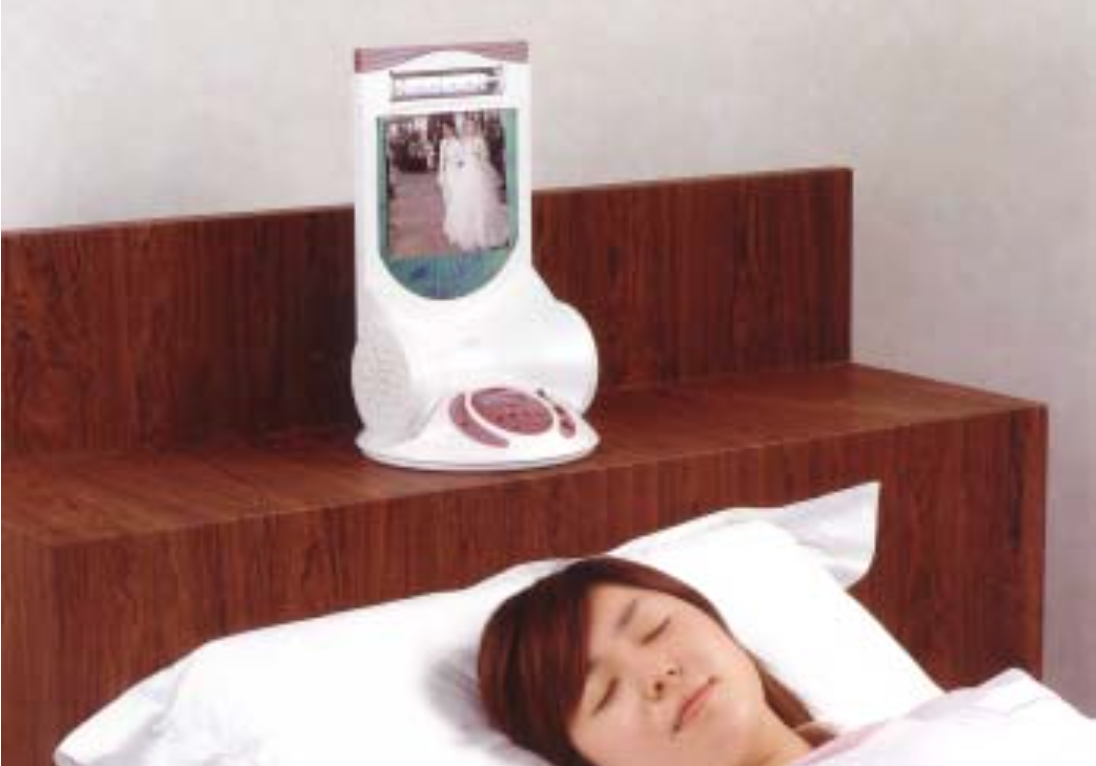
\includegraphics[width=7cm]{eps/takaratomi.eps}
\caption{DreamOnレビュー}
\label{DreamOnレビュー}
\end{center}
\end{figure}


\subsection{iWinks}
\begin{itemize}
\item 目的:睡眠と光や音との関係性を活用し睡眠深度に即 した刺激を与える抱き枕型のインタフェースの提案 \cite{iWinks}
\item 正確性:モニタリングについてはアプリと照合されてある程度の正確性は証明されているが、光の部分については実験結果が明らかになっていない。
\item インプット:睡眠にゆかりのあるインターフェースである枕の改良を行うことで、新しいインタフェースの提案をしているが、その効果は実証されていない。
\item 値段:商業用目的ではないため不明
\end{itemize}

\subsection{DreamOn}
\begin{itemize}
\item 概要:スマートフォンアプリ、健康のカテゴリーに属す。レーティングは3であり、385のレーティングが残っている。
\item 目的:アプリという形で多くの人に夢の研究に参加してもらい音が夢に影響を与えるのか否かについて判明する。 \cite{dreamOn}
\item 効果:睡眠は外的刺激に影響を受ける。例えば森林の音を流すと夢の中に緑が頻繁に現れて、街中の音を流すと奇抜な夢を見るとかいてある。
\item 正確性:アプリの実験をしてもらおうと試みがあったが実験結果についてはかなり疑わしい。かきの画像はユーザーのレビューである。悪夢を見たなどの、睡眠被害を訴えるレビューが多く見受けられた。
\item インプット:音
\item 値段:無料であるが、音声の中には有料のものも有る。
\end{itemize}

\begin{figure}[htbp]
\begin{center}
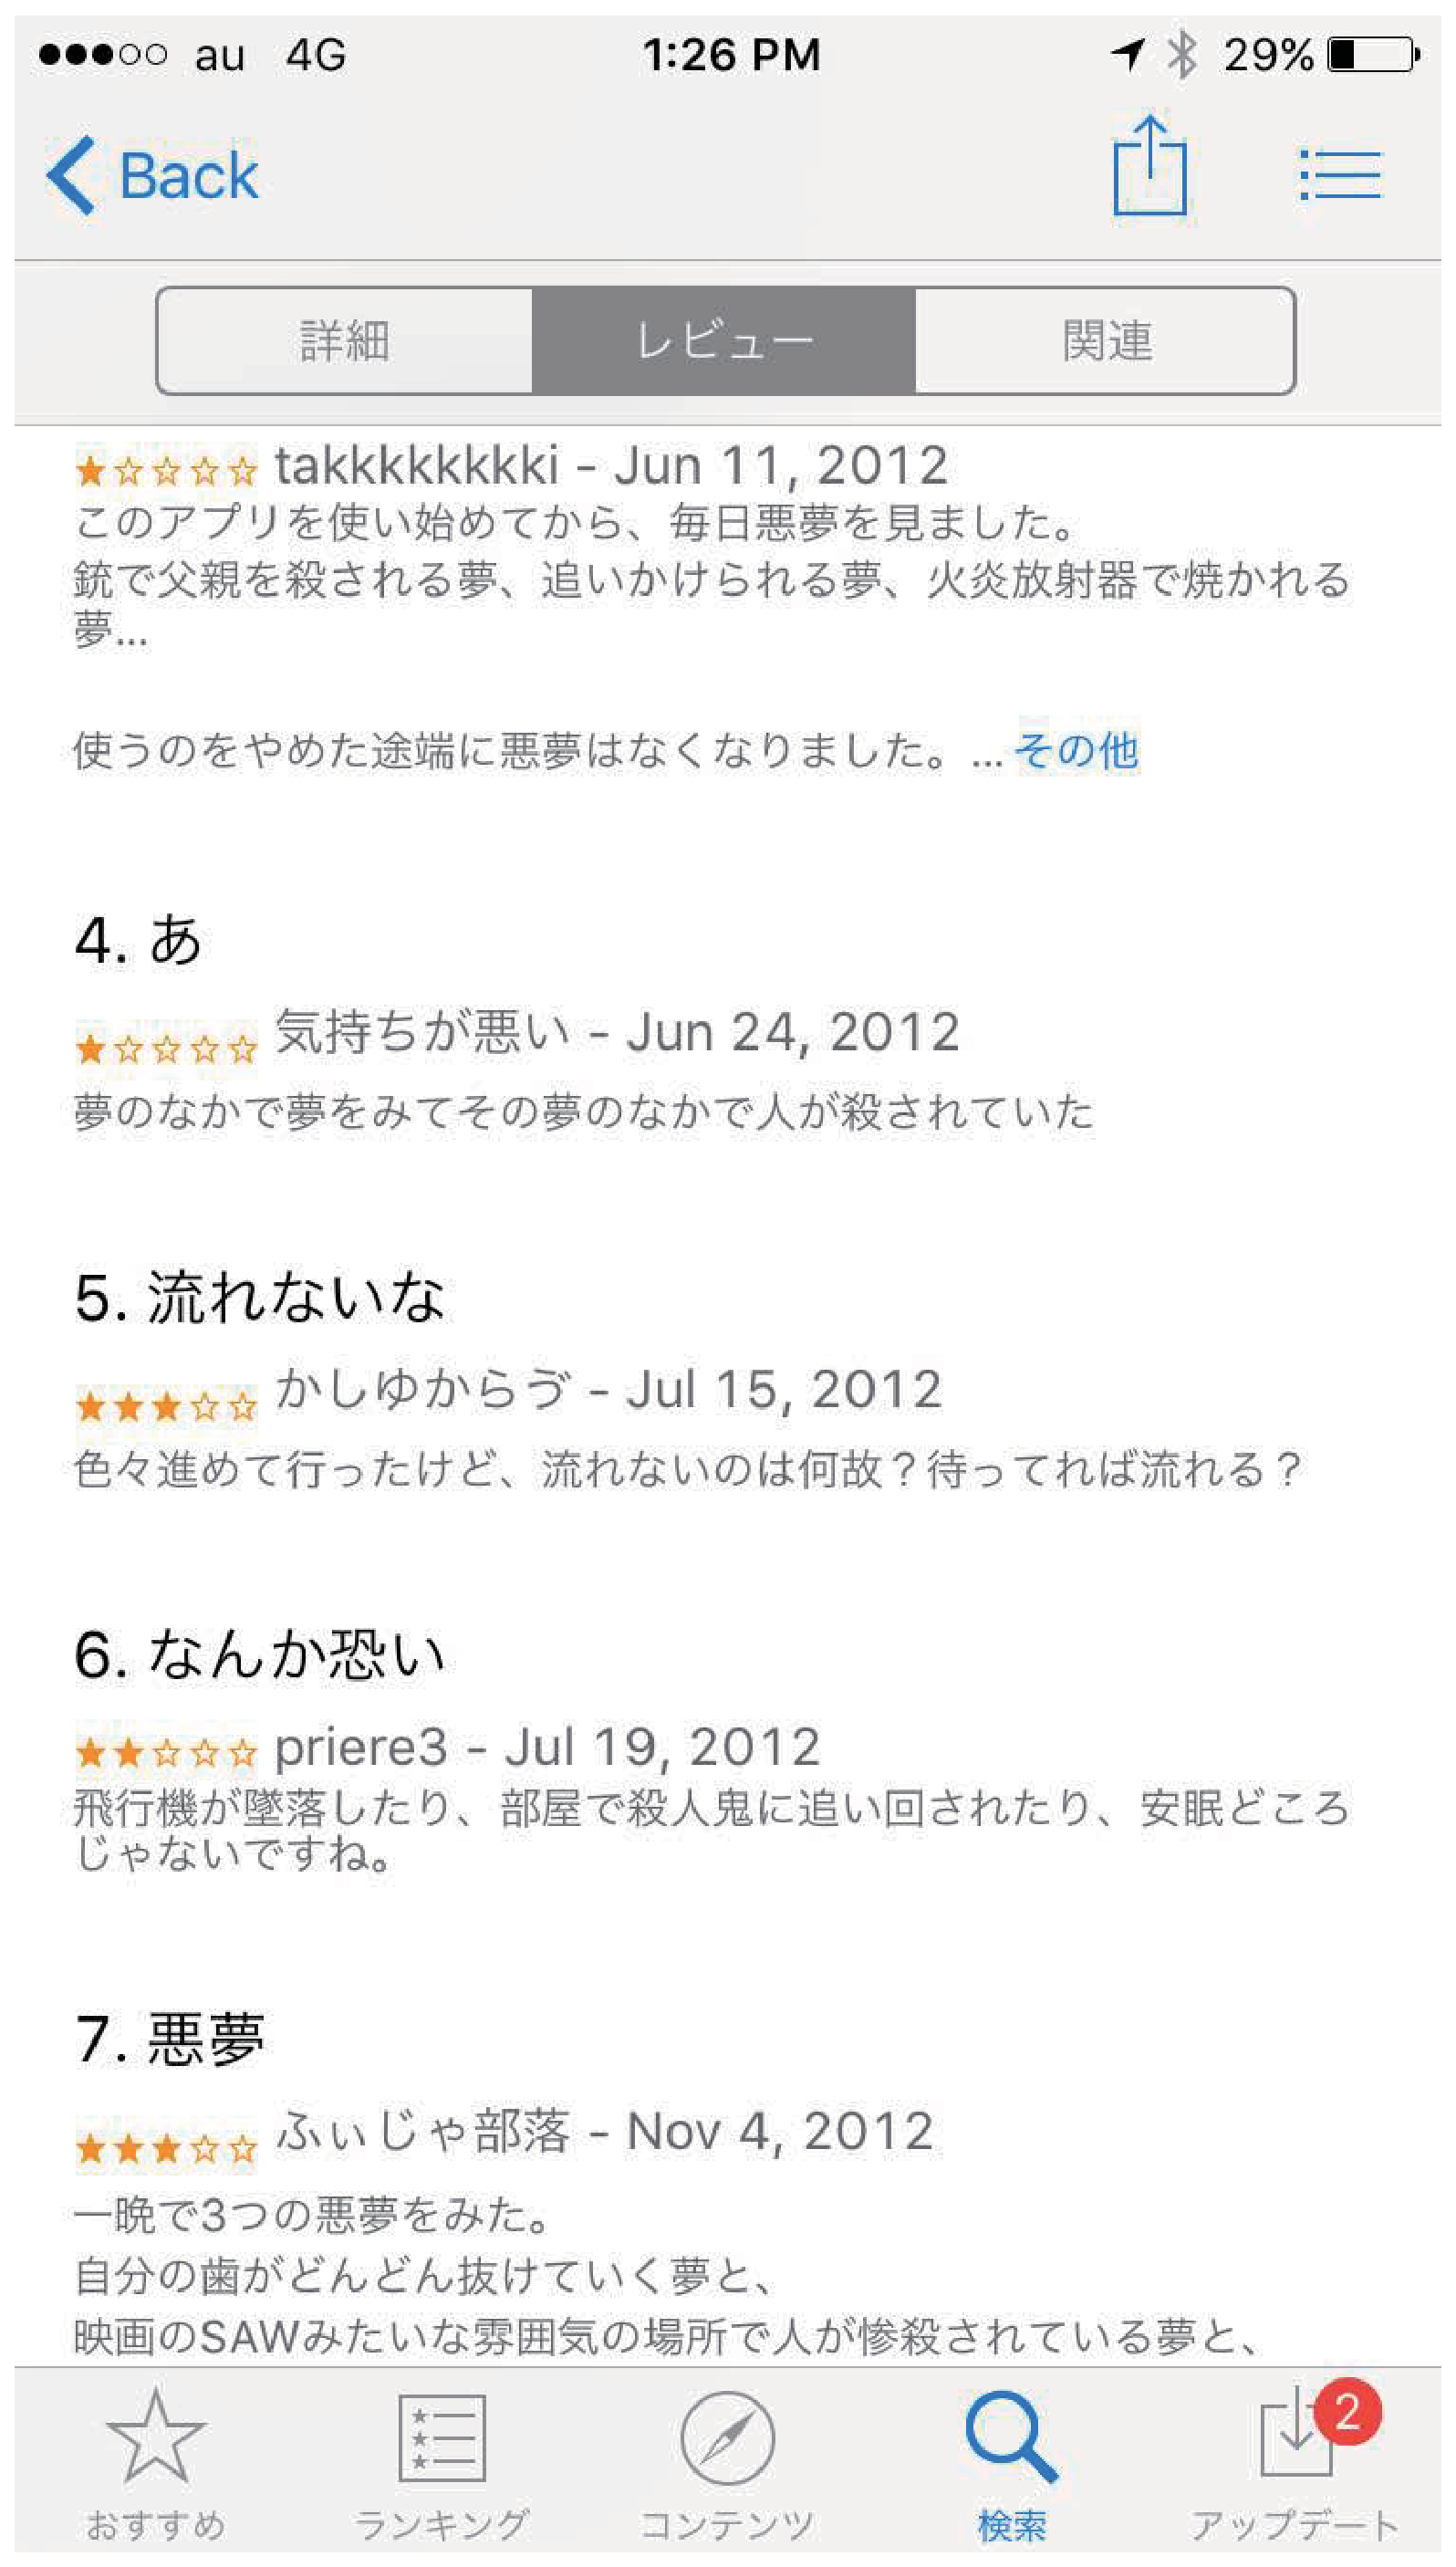
\includegraphics[width=7cm]{eps/dreamOn.eps}
\caption{DreamOnレビュー}
\label{DreamOnレビュー}
\end{center}
\end{figure}

\section{MemoryDreamの立ち位置}
夢を操作するために多くの研究が行われてきたが、実験結果については明らかになっていない。以下の先行研究を参考にしてMemoryDreamは以下の点を明確にしたい。
\begin{itemize}
\item 実験結果が明快かつ詳しい
\item コストのかかるデバイスを必要としない
\item ユーザーによってカスタマイズが容易であること
\end{itemize}

%\section{先行研究}
%当研究室にて行われた研究として、以下の研究がある。

%\subsection{e-learningコンテンツにおけるドキュメントサーチの最適化\cite{docsearch}}
%Yahoo!Search BOSS APIを用いて、有用なWebページへのヒット率を向上させる実験が行われた。その結果、検索を行う主なキーワードとは別に、HTMLページ中に埋め込まれた<meta>タグのkeyword属性のパラメータとして特に多いものをサブキーワードとして検索を行う方法にて、有用なWebサイトへのヒット率が向上することが確認された。

%\section{サブキーワードの選出}
%上記研究結果から、e-learningコンテンツへのアクセス精度を高めるため、サブキーワードを選出する方法を考える。

%\subsection{選出過程}
%サブキーワードを選出する方法に上記の先行研究結果を用いることを試みたのだが、HTMLをキャッシュせず、検索を行うたびに毎回数十ページへアクセスを行なっていたため、タブレット端末やスマートフォン端末など、通信が不安定になる可能性が高い端末でこれを用いることは難しいと判断した。よって今回は、予めヒット率が向上すると考えられるキーワードを適当に予測、検証し、1〜2個程度のサブキーワードを選出した。

%\subsection{選出結果}
%\begin{itemize}
%\item 基礎
%\item 講座
%\end{itemize}
%以上の2個をサブキーワードとする。サブキーワードはORに設定して検索を行い、どちらか片方が、メインキーワードと共にヒットした場合の結果のみを引き出すよう設定する。この手法により、e-learningコンテンツのみに絞った検索結果をwebAPIより得られるよう構成した。 